% Template for NIME 2023

% Modified by Adnan Marquez-Borbon 30 November 2022
% Modified by Courtney Reed 28 November 2022
% Modified by Joe Wright 14 December 2019
% Modified by Niccolò Granieri 10 October 2018 
% Modified by Angelo Fraietta 23 December 2018
% Modified by Angelo Fraietta 22 November 2018
% Modified by Rodrigo Schramm on 22 September 2018
% Modified by Luke Dahl on 17 October 2-17
% Modified by Cumhur Erkut on <2016-10-11 Tue>
% Modified by Edgar Berdahl on 5 November 2014
% Modified by Baptiste Caramiaux on 25 November 2013
% Modified by Kyogu Lee on 7 October 2012
% Modified by Georg Essl on 7 November 2011
%
% Based on "sig-alternate.tex" V1.9 April 2009
% This file should be compiled with "nime-alternate.cls"

\documentclass{nime-alternate_ADJ} % license and conference information box reduced a bit
% \documentclass{nime-alternate} % Uncomment when publishing final version
% \documentclass{nime-alternate_MANUSCRIPT} % remove conference information

% Uncomment only one of the ones below
\usepackage{anonymize} 		   %Uncomment this line to publish
% \usepackage[blind]{anonymize}%Uncomment this line for blind review

% Package that enables the use of accents and non 
% standard characters
\usepackage[utf8]{inputenc}

\usepackage[implicit=false]{hyperref}

\begin{document}

% --- Author Metadata here ---
%\conferenceinfo{NIME'17,}{May 15-19, 2017, Aalborg University Copenhagen, Denmark.}
%\conferenceinfo{NIME'18,}{June 3-6, 2018, Blacksburg, Virginia, USA.}
%\conferenceinfo{NIME'19,}{June 3-6, 2019, Federal University of Rio Grande do Sul, ~~~~~~  Porto Alegre,  Brazil.}
% \conferenceinfo{NIME'20,}{July 21-25, 2020, Royal Birmingham Conservatoire, ~~~~~~~~~~~~ Birmingham City University, Birmingham, United Kingdom.}
%\conferenceinfo{NIME'22,}{June 28 - July 1, 2022, Waipapa Taumata Rau, T\={a}maki ~~~~~~~~ Makaurau, Aotearoa}

\conferenceinfo{NIME'23,}{31 May–2 June, 2023, Mexico City, Mexico.}

\title{Delayed Gestural Control of Musical Sound \\
using Online Unsupervised Temporal Segmentation: \\
Brief Report}

% You need the command \numberofauthors to handle the 'placement
% and alignment' of the authors beneath the title.
%
% For aesthetic reasons, we recommend 'three authors at a time'
% i.e. three 'name/affiliation blocks' be placed beneath the title.
%
% NOTE: You are NOT restricted in how many 'rows' of
% "name/affiliations" may appear. We just ask that you restrict
% the number of 'columns' to three.
%
% Because of the available 'opening page real-estate'
% \label{key}% we ask you to refrain from putting more than six authors
% (two rows with three columns) beneath the article title.
% More than six makes the first-page appear very cluttered indeed.
%
% Use the \alignauthor commands to handle the names
% and affiliations for an 'aesthetic maximum' of six authors.
% Add names, affiliations, addresses for
% the seventh etc. author(s) as the argument for the
% \additionalauthors command.
% These 'additional authors' will be output/set for you
% without further effort on your part as the last section in
% the body of your article BEFORE References or any Appendices.

\numberofauthors{1} %  in this sample file, there are a *total*
% of EIGHT authors. SIX appear on the 'first-page' (for formatting
% reasons) and the remaining two appear in the \additionalauthors section.
%
\author{
% You can go ahead and credit any number of authors here,
% e.g. one 'row of three' or two rows (consisting of one row of three
% and a second row of one, two or three).
%
% The command \alignauthor (no curly braces needed) should
% precede each author name, affiliation/snail-mail address and
% e-mail address. Additionally, tag each line of
% affiliation/address with \affaddr, and tag the
% e-mail address with \email.
%
% 1st. author
\alignauthor
\anonymize{Juan Ignacio Mendoza}\\
%       \affaddr{\anonymize{University of Jyväskylä, Finland}}\\ % Jyväskylä Jyvaskyla
       \affaddr{\anonymize{University of Jyväskylä}}\\ % Jyväskylä Jyvaskyla
 %             \affaddr{\anonymize{University of Jyvaskyla}}\\ % Jyväskylä Jyvaskyla
      \affaddr{\anonymize{Finland}}\\
      \email{\anonymize{juigmend@student.jyu.fi}}
%% 2nd. author
%\alignauthor
%\anonymize{G.K.M. Tobin}\titlenote{\anonymize{The secretary disavows
%any knowledge of this author's actions.}}\\
%       \affaddr{\anonymize{Institute for Clarity in Documentation}}\\
%       \affaddr{\anonymize{P.O. Box 1212}}\\
%       \affaddr{\anonymize{Dublin, Ohio 43017-6221}}\\
%       \email{\anonymize{webmaster@marysville-ohio.com}}
%% 3rd. author
%\alignauthor \anonymize{Lars Th{\o}rv{\"a}ld}\titlenote{This author is the
%one who did all the really hard work.}\\
%       \affaddr{\anonymize{The Th{\o}rv{\"a}ld Group}}\\
%       \affaddr{\anonymize{1 Th{\o}rv{\"a}ld Circle}}\\
%       \affaddr{\anonymize{Hekla, Iceland}}\\
%       \email{l\anonymize{arst@affiliation.org}}
%\and  % use '\and' if you need 'another row' of author names
%% 4th. author
%\alignauthor \anonymize{Lawrence P. Leipuner}\\
%       \affaddr{\anonymize{Brookhaven Laboratories}}\\
%       \affaddr{\anonymize{Brookhaven National Lab}}\\
%       \affaddr{\anonymize{P.O. Box 5000}}\\
%       \email{\anonymize{lleipuner@researchlabs.org}}
%% 5th. author
%\alignauthor \anonymize{Sean Fogarty}\\
%       \affaddr{\anonymize{NASA Ames Research Center}}\\
%       \affaddr{\anonymize{Moffett Field}}\\
%       \affaddr{\anonymize{California 94035}}\\
%       \email{\anonymize{fogartys@amesres.org}}
%% 6th. author
%\alignauthor \anonymize{Anon Nymous}\\
%       \affaddr{\anonymize{Redacted }}\\
%       \affaddr{\anonymize{8600 Datapoint Drive}}\\
%       \affaddr{\anonymize{San Antonio, Texas 78229}}\\
%       \email{\anonymize{cpalmer@prl.com}}
}
% There's nothing stopping you putting the seventh, eighth, etc.
% author on the opening page (as the 'third row') but we ask,
% for aesthetic reasons that you place these 'additional authors'
% in the \additional authors block, viz.
%\additionalauthors{Additional authors: \anonymize{John Smith (The Th{\o}rv{\"a}ld Group,}
%email: {\texttt{\anonymize{jsmith@affiliation.org}}}) and \anonymize{Julius P.~Kumquat 
%(K. Consortium,} email: {\texttt{\anonymize{jpkumquat@consortium.net}}}).}
%\date{30 July 1999}
% Just remember to make sure that the TOTAL number of authors
% is the number that will appear on the first page PLUS the
% number that will appear in the \additionalauthors section.

% For your initial submission you MUST ANONYMIZE the authors.

\maketitle

\begin{abstract}
The state-of-the-art recognition of continuous gestures for control of musical sound by means of machine learning has two notable constraints. The first is that the system needs to be trained with individual example gestures, the starting and ending points of which need to be well defined. The second constraint is time required for the system to recognise that a gesture has occurred, which may prevent the quick action that musical performance typically requires. This article describes how a method for unsupervised segmentation of gestures, may be used for delayed gestural control of a musical system. The system allows a user to perform without explicitly indicating the starting and ending of gestures in order to train the machine learning algorithm. To demonstrate the feasibility of the system, an apparatus for control of musical sound was devised incorporating the time required by the process into the interaction paradigm. The unsupervised automatic segmentation method and the concept of delayed control are further proposed to be exploited in the design and implementation of systems that facilitate seamless human-machine musical interaction without the need for quick response time, for example when using broad motion of the human body.
%\vspace{0.5cm}
\end{abstract} 
\keywords{unsupervised, segmentation, machine learning, gesture, recognition, accelerometry, music, controller, interface, DMI}
%\vspace{0.5cm}

% ------- CCS Concepts
% Here is where you enter the CCS Concepts for your paper.
%
% It is strongly recommended that authors view the submission form
% prior to starting to write the paper, which includes information 
% on the CCS Concepts. 
% 
% The 2012 ACM Computing Classification System (CCS) replaces the
% traditional 1998 version, which has served as the de facto 
% standard classification system for the computing field. It is
% being integrated into the search capabilities and visual topic 
% displays of the ACM Digital Library. Please enter the CCS XML code 
% for the classification terms that describe your paper. To get the 
% XML code, please use the following procedure, which is
% demonstrated using three NIME-related example terms: Applied
% computing~Sound and music computing, Applied computing~Performing
% arts, and Information systems~Music retrieval.
%
% 1) Browse to the website http://dl.acm.org/ccs_flat.cfm.
% 2) Select one to three classification terms from the website that
%    describe your paper (e.g. for the example paper Applied
%    computing~Sound and music computing, Applied 
%    computing~Performing arts, and Information systems~Music
%    retrieval.).
% 3) For each classification you need to select the relevance
%    (e.g. for this example, Sound and music computing is "high",
%    Performing arts is "low", and Music retrieval is "Medium")
% 4) Once you have selected the last term, click on "view CCS Tex
%    Code". This will generate some code, which includes some CCSXML
%    and some lines beginning with \ccsdesc.
% 5) Keep all of this code, as you will need it for entering into
%    the Precision Conference System paper submission form.
% 6) For this document, keep only the \ccsdesc lines. Here is what
%    you would paste for the classification example:

\ccsdesc[500]{Computing methodologies~Machine learning}
\ccsdesc[500]{Applied computing~Sound and music computing}
\ccsdesc[100]{Applied computing~Performing arts}
\ccsdesc[100]{Information systems~Music retrieval}

% this line creates the CCS Concepts section.
\printccsdesc
%\vspace{1cm}

\section{Introduction}

Musical instruments are usually designed to be controlled with fine movements of hands and fingers, as they afford precision and speed. These qualities are often described as the foundations of responsiveness, believed to be indispensable for musical expression. The instrument thus becomes an extension of the human body. 

These ideas have permeated into the design of digital musical instruments (DMI) \cite{Moore_1988}, and a response time approaching zero has become a standard goal \cite{Wessel_Wright_2002, Jack_etal_2018, McPherson_etal_2016}. The challenge extends to the design of DMI that recognise gestures ``in the air", using machine learning techniques. For example, a musician wears, holds or stands in front of, a device that may sense position (i.e., static gestures) or motion (i.e., continuous gestures). The musician makes a gesture in free space, for example describes a circle with the head, or wiggles a hand, or stands in a particular pose. The DMI learns these gestures in a process called ``training", and it recognises them when they are performed. The recognition of a gesture can be mapped to a musical action, such as triggering a sound, activating an effect, etc. (e.g., \cite{Gillian_2011}).

Two algorithms and variations of them have been extensively used to recognise continuous gestures, regardless of the sensing technology: Dynamic Time Warping (DTW) \cite{Gillian_etal_2011} and Hidden Markov Models (HMM) \cite{Bevilacqua_etal_2010}. Both estimate the likelihood that a gesture being performed corresponds to a gesture that has been learned in the training. However, this likelihood may change while the gesture is executed, therefore recognition is only reliable after the gesture has been completed. This adds time to the recognition, arguably reducing responsiveness. In addition, training requires the beginning and ending of gestures to be explicit.

Given a stream of data from a sensor, individual gestures may be extracted by a process called ``segmentation", in which the start and ending points of gestures are identified. For example, when training the algorithm the user presses a button (e.g., \cite{Merril_Paradiso_2005}) or makes pauses between gestures (e.g., \cite{Murad_etal_2017}). While this constraint has not prevented the use of the algorithms mentioned above in DMI, the ability of a machine to recognise and learn gestures without explicit training would open new avenues for human-machine musical interaction. Furthermore, the time required for the recognition of continuous gestures might not be a disadvantage if when designing a DMI we don't hold the same standards of responsiveness as for the human voice or other non-electronic instruments. Consider that digital technologies have greatly expanded our possibilities for control of sound, far beyond what is possible with the human voice or with non-electronic devices. Why should we hold ourselves from exploring forms of gestural control that are not quick and precise, but instead slow and imprecise (delayed detection, perception, action, by the user and the automatic system) such as broad motion of the human body?
	
This article describes a system that was devised as a proof of concept towards exploring the feasibility of unsupervised learning of patterns in a continuous input signal, in a musical application that doesn't require quick responsiveness. The system is conceptually a musical instrument in a broad sense, for it essentially allows a user to control sound.

\section{Online Unsupervised Temporal Segmentation}\label{OUTS}

A signal may be segmented using the algorithm described by Foote \cite{Foote_2000}, which has seen application in segmentation of musical audio and video \cite{Foote_Cooper_2003, Tardieu_etal_2009}, dancing motion captured by an accelerometer \cite{Mendoza_Thompson_2017}, and daily activity recorded by wearable accelerometers \cite{Mendoza_etal_2022, Rodrigues_Probst_Gamboa_2021}. Its meta-parameters can be adjusted to detect boundaries of segments at different timescales. The cited sources described the use of the algorithm on recorded data. Conversely, Schätti \cite{Schatti_2007} described an online version of the algorithm, that detects boundaries of audio data while the data is being produced. Later  
% \anonymize{foooooooooooooooooo}
Mendoza \cite{Mendoza_2022} 
reported a study in which the algorithm's segmentation of dancing motion captured by a hand-held accelerometer, was compared to manual segmentation of video recordings of the dancing. The meta-parameters were optimised for each accelerometry recording. The music used for  dancing and the person doing the manual segmentation were the main factors affecting the quality of computed segmentation. These results suggest that the algorithm is suitable for gestural control of a DMI, albeit its meta-parameters might need contextual adjustment. Figure~\ref{fig_1} succinctly illustrates the online segmentation procedure. It uses the same principle of buffering and computation of a local distance matrix, as described by Schätti \cite{Schatti_2007} and 
% \anonymize{foooooooooooooooooo}
Mendoza \cite{Mendoza_2022}.

\begin{figure}[ht!]
	\centering
		%\includegraphics[trim={1cm 1.4cm 1cm 5.6cm}, clip=true, width=1\columnwidth]{fig_1}
		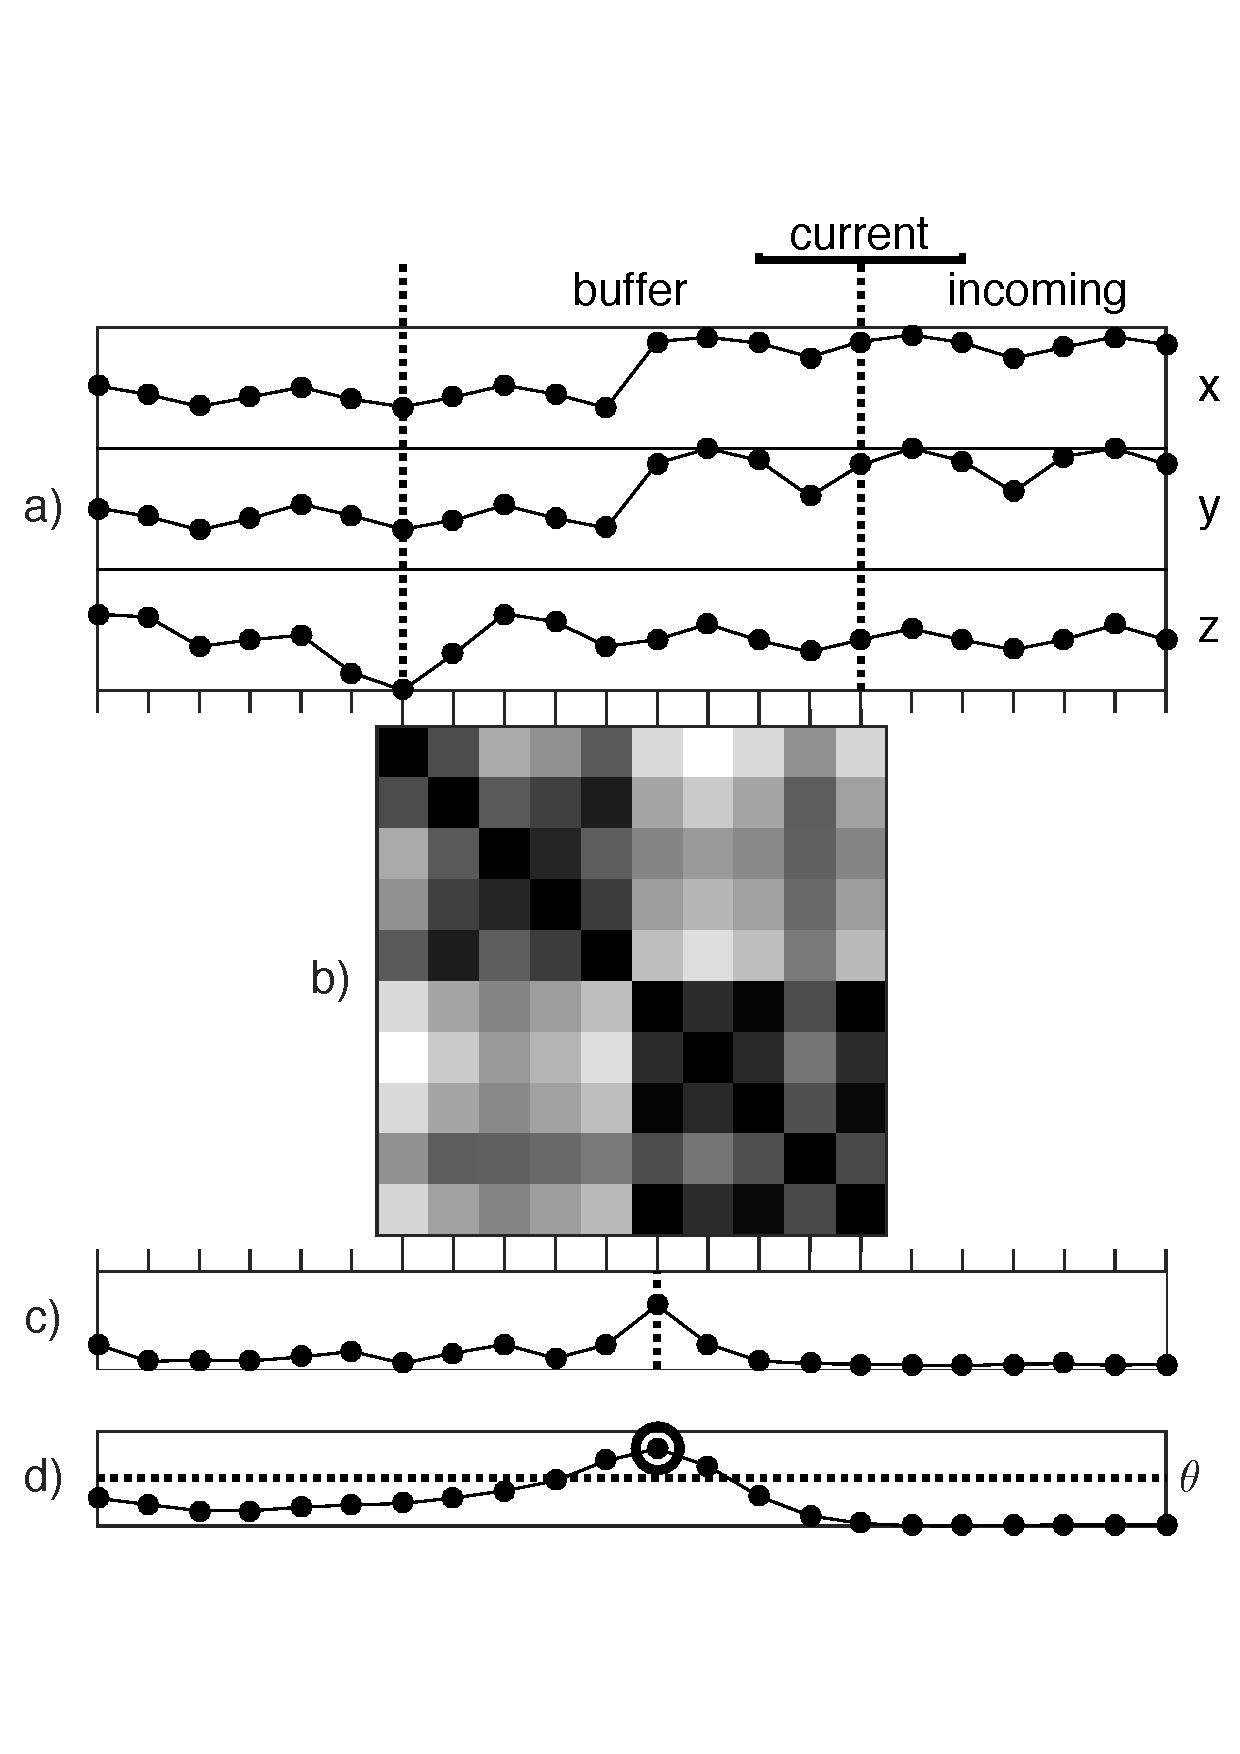
\includegraphics[trim={0.3cm 3.5cm 0.3cm 3.5cm}, clip=true, width=1\columnwidth]{fig_1_LO}
		% 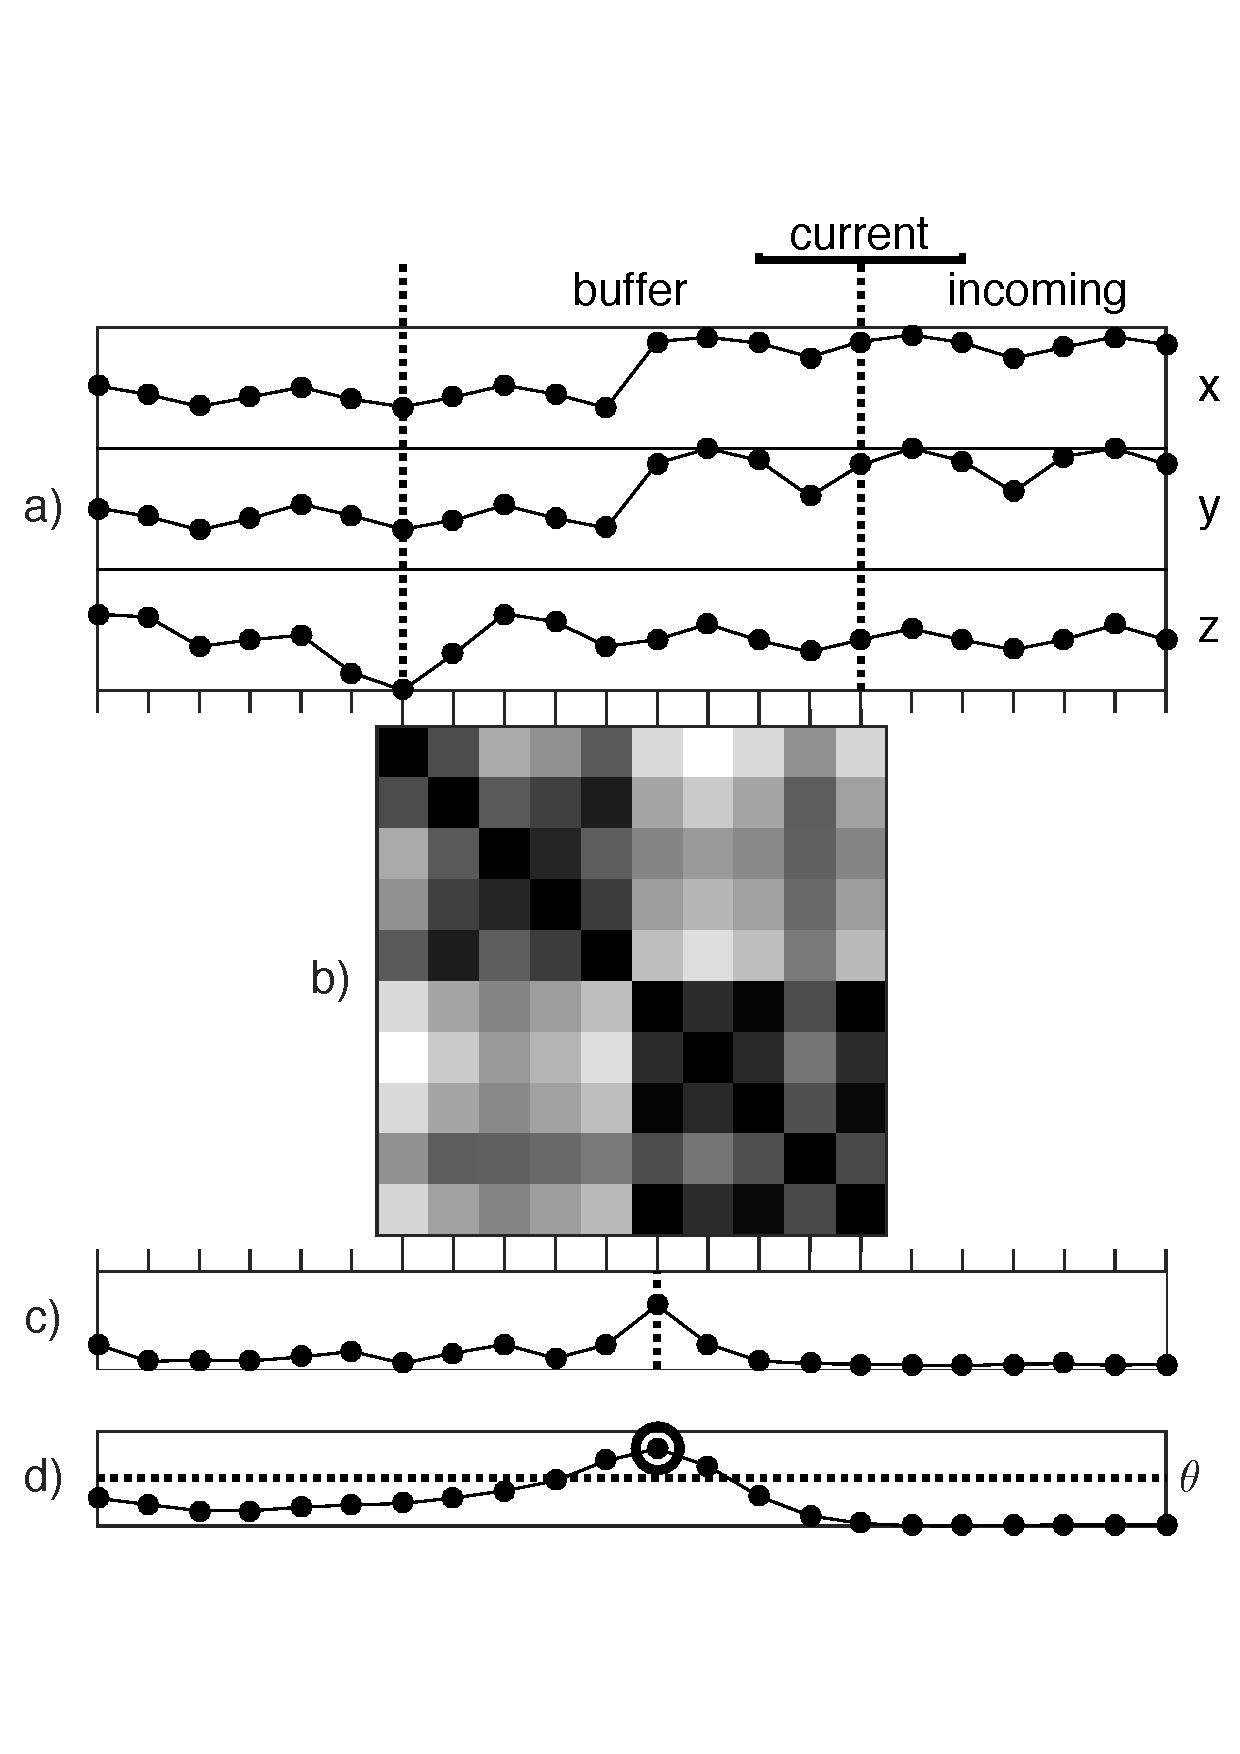
\includegraphics[width=1\columnwidth]{fig_1_LO}
	\caption{Online temporal segmentation. Horizontal axes represent time. (a) is accelerometer data composed of triaxial frames. (b) is a distance matrix of the data in the buffer having a length of $n$ frames. Lighter shades represent more distance. (c) is a novelty score resulting from the correlation of the distance matrix with a gaussian-tapered checkerboard kernel. The vertical dotted line indicates the current result. (d) is the novelty score after smoothed by a low-pass filter of length $n_{filt}$, where $\theta$ is a threshold and the point in a circle is the selected peak indicating a  boundary. Note that this visualisation shows (c) and (d) aligned in time, but in practice there will be a lag because of the filter. The total lag of the process is $(n+ n_{filt})/2$ frames plus 3 frames for peak detection.}
	\label{fig_1}
\end{figure}

\section{Proof of Concept}

\subsection{Hardware}

A polystyrene ball having 12 cm. of diameter was cut in half and the interior was carved to fit a Myo armband controller (Figure~\ref{fig_2}). The Myo was originally designed by Thalmic Labs to be worn on the forearm. It has several sensors, of which only its triaxial accelerometer was used in the system described here. The two halves of the ball are put together restoring the spherical shape, but it can be easily disassembled to recharge the battery of the Myo. The data from the sensors is broadcast in real time using the Bluetooth Low-Energy (BLE) specification. The BLE signal is captured by a computer nearby, and a piece of software by Rodrigo Schramm\footnote{See~\cite{Visi_2017}.~Software~available:~\href{https://github.com/federicoVisi/KineToolbox/blob/master/input\%2BML/DaemonMYO}{https://github.com/federicoVi\\si/KineToolbox/blob/master/input\%2BML/DaemonMYO}} outputs the data in Open Sound Control (OSC) format to a User Datagram Protocol (UDP) port, where it can be accessed by other software. This controller was used for its convenience, as it was available to the researcher along with the software to get the data in real time.

\begin{figure}[t!]
   \setlength\tabcolsep{2pt} 
    \begin{tabular}{cc}
        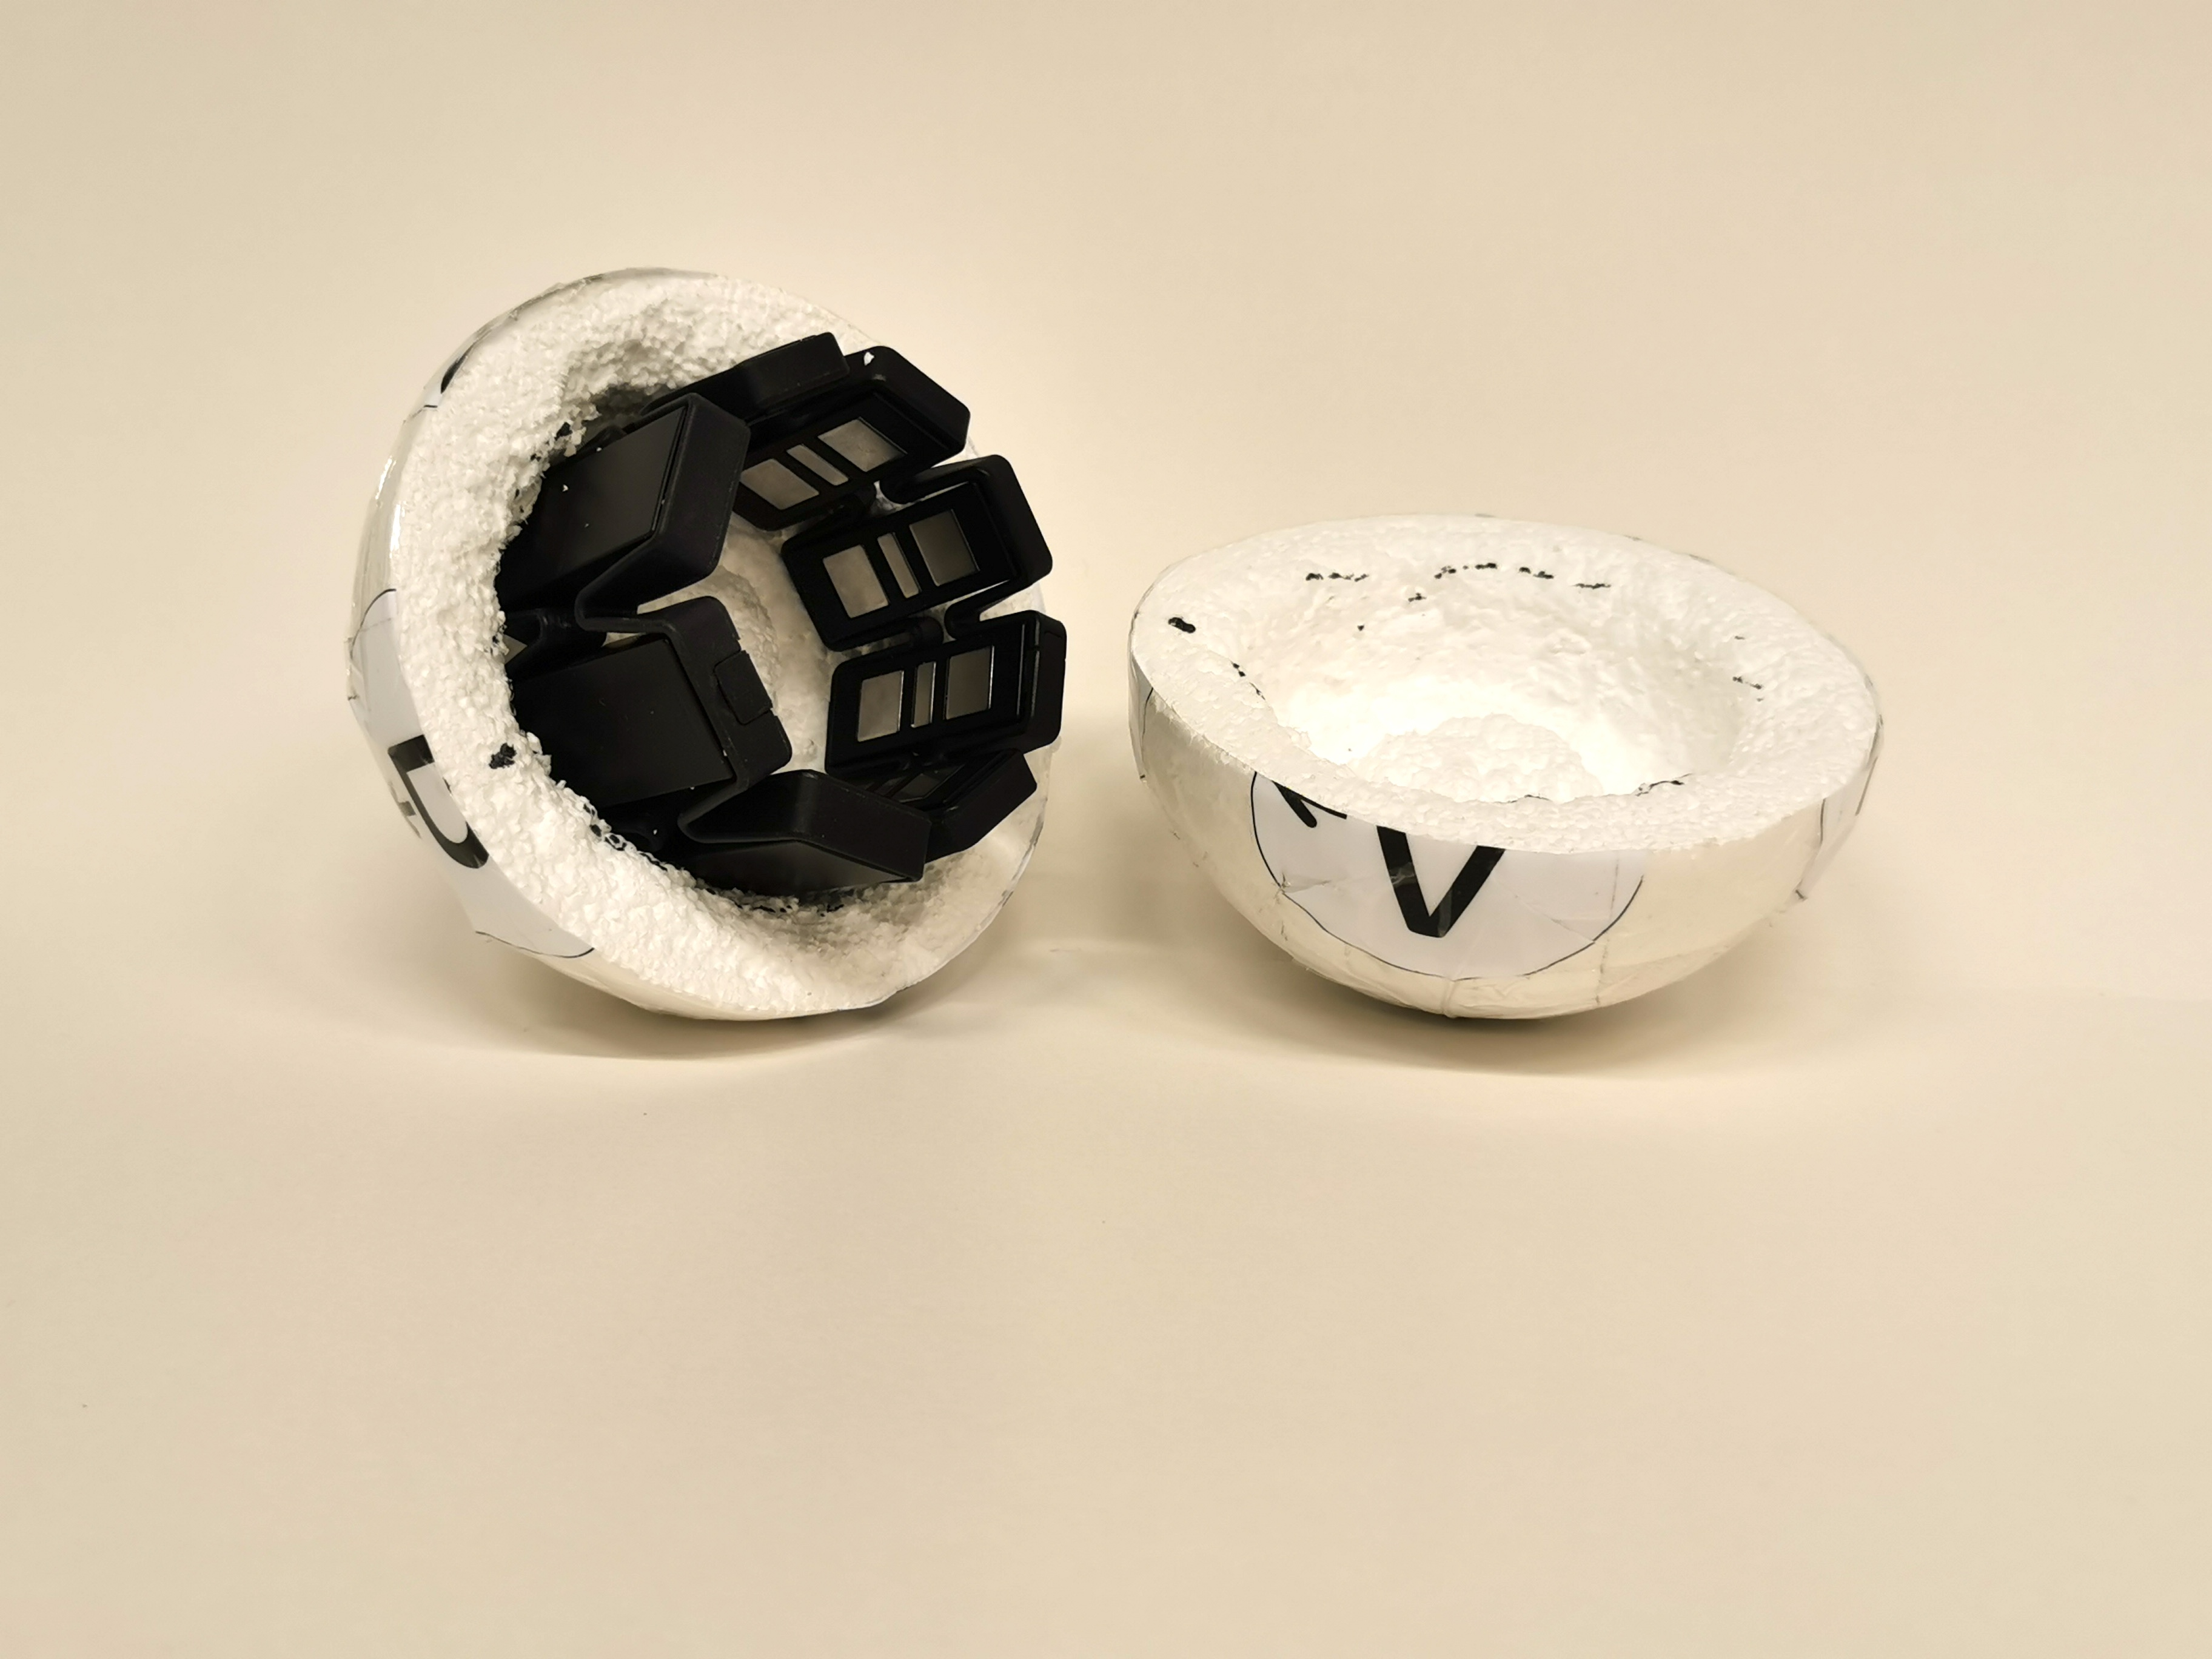
\includegraphics[trim={10cm 24cm 10cm 6cm}, clip=true, width=0.48\columnwidth]{ball_open}
        &
        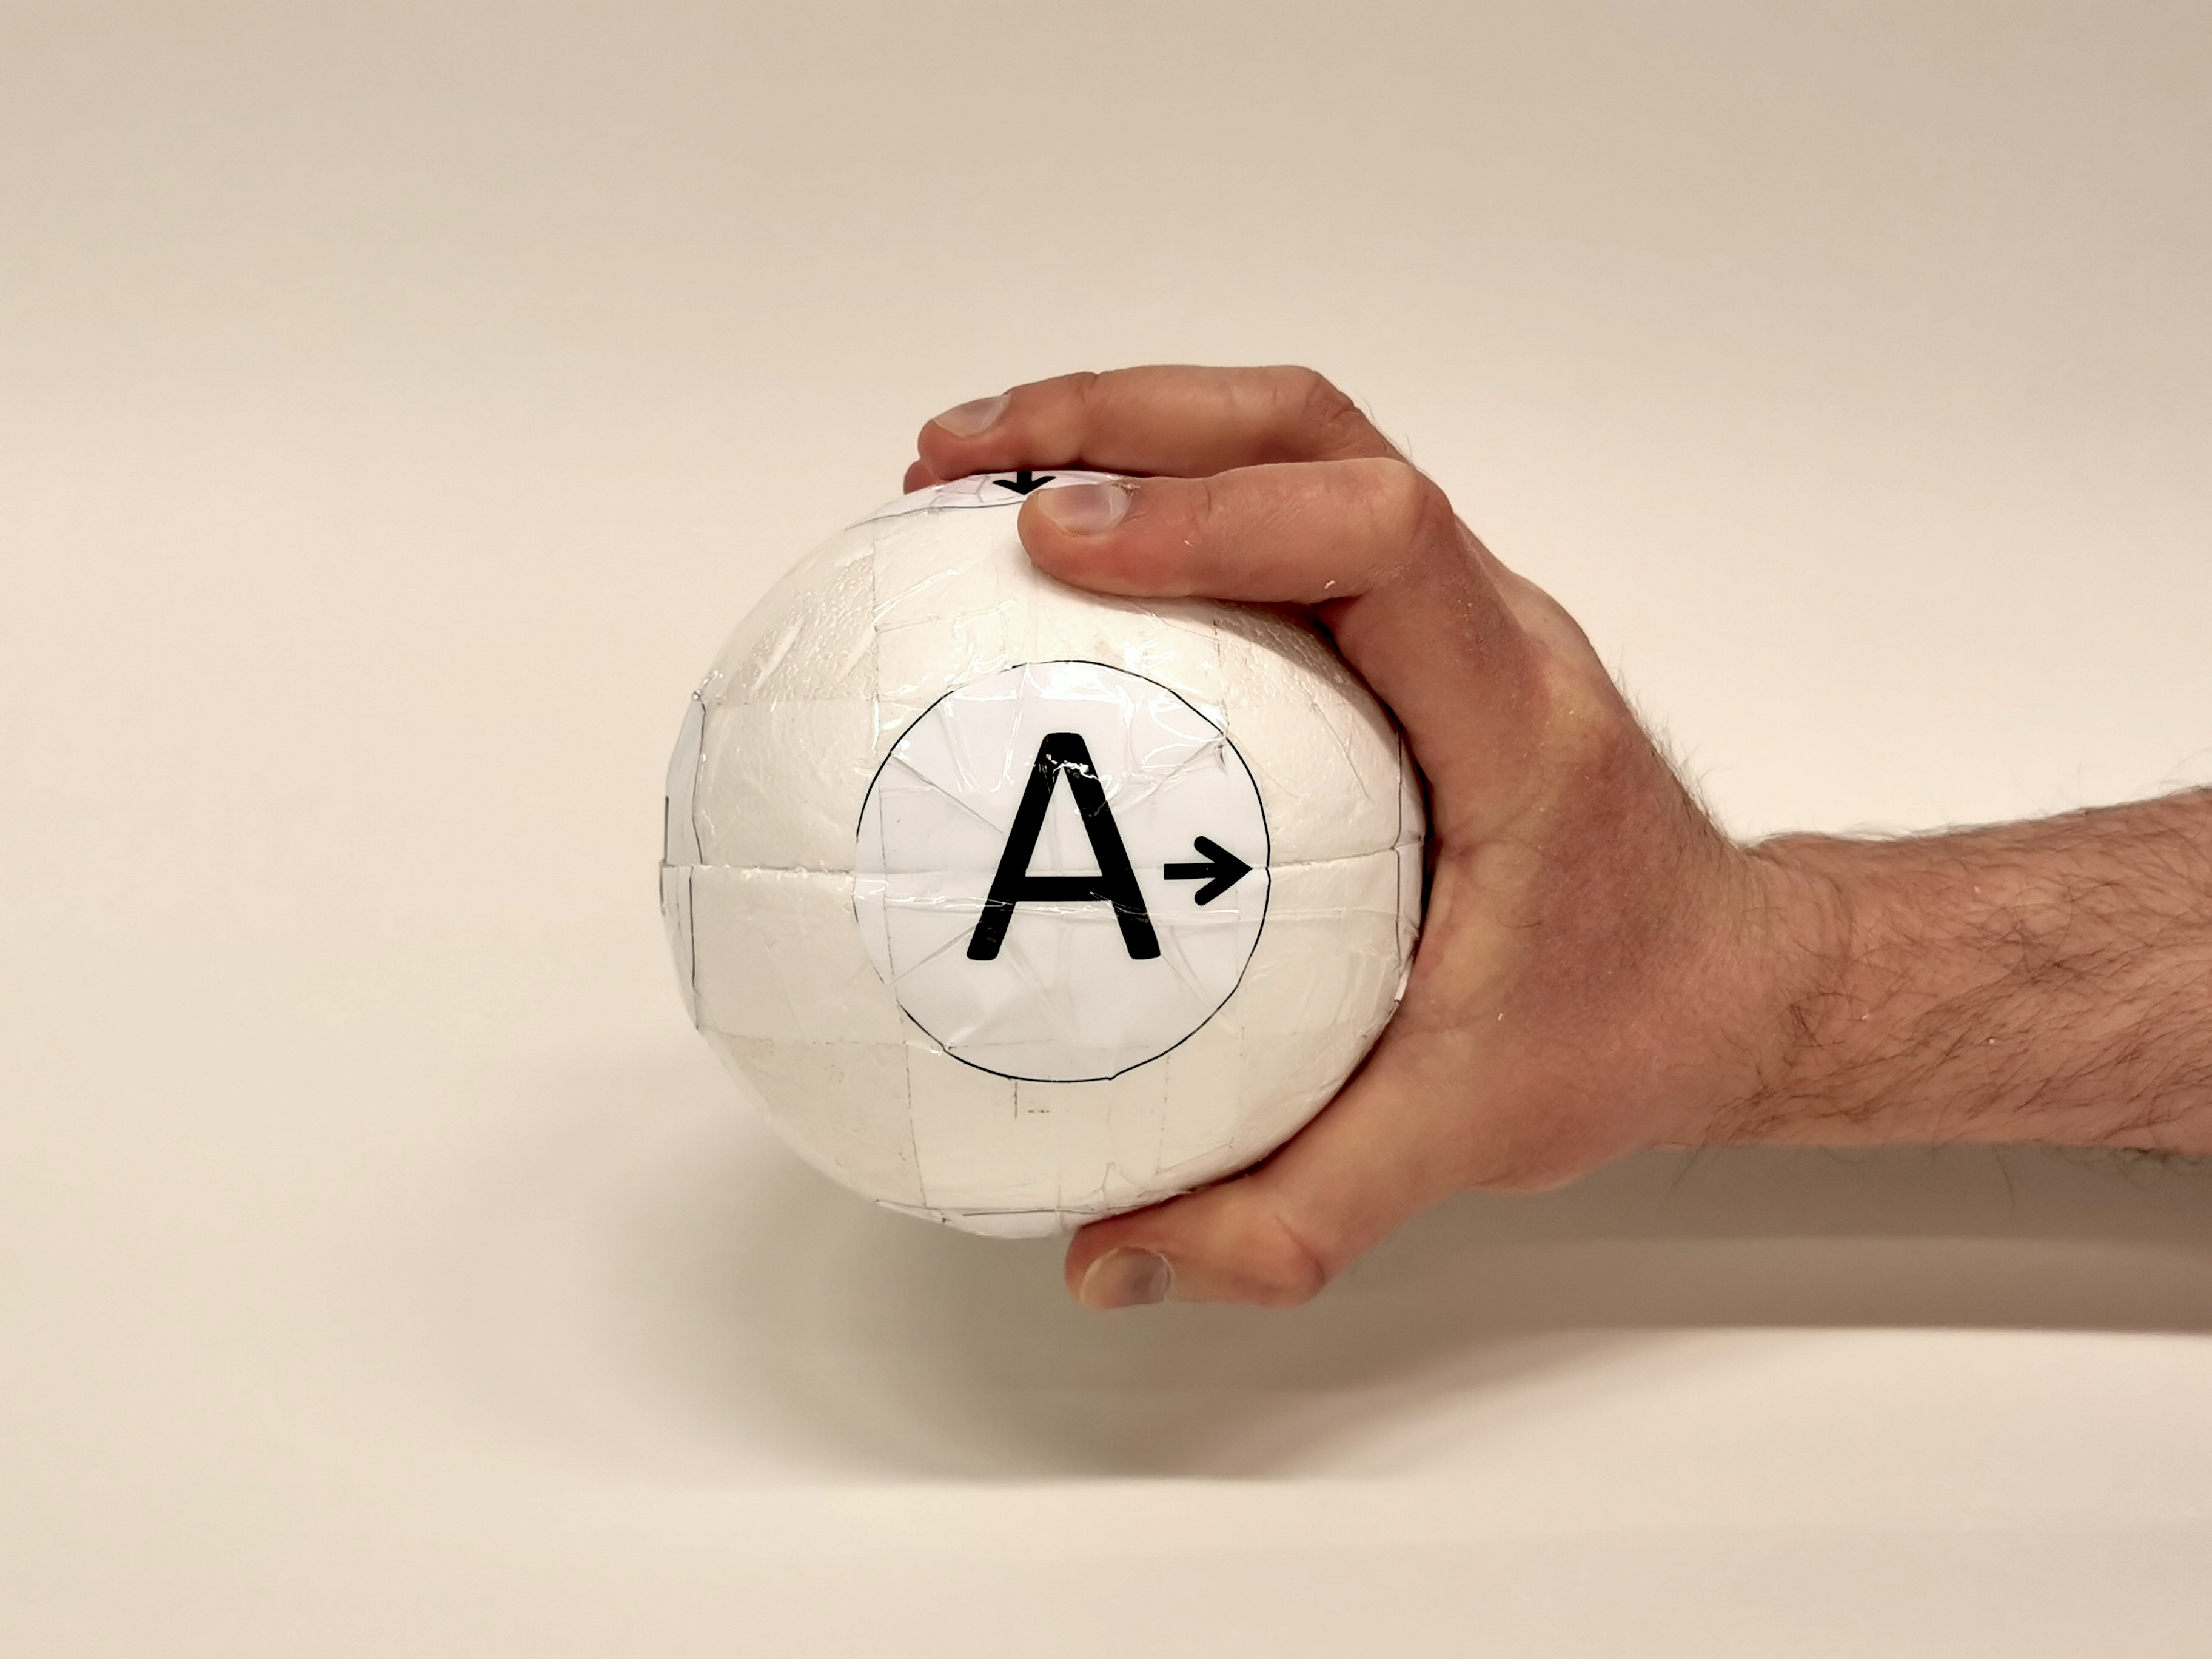
\includegraphics[trim={20cm 15cm 0cm 15cm}, clip=true, width=0.48\columnwidth]{ball_handheld}
    \end{tabular}
	\caption{Left -- Carved open polystyrene ball with the Myo armband in it. Right -- Closed ball.}
	\label{fig_2}
\end{figure}

\subsection{Software}

The segmentation procedure described in section \ref{OUTS} can detect in real-time boundaries between gestures performed with the hand-held controller continuously, without indicating their start or end.  The effect of its meta-parameters are as follows: $n$  sets the timescale of gestures to detect, $n_{filt}$ sets the smoothness of the novelty score, $\theta$ is a factor of the maximum novelty score and sets a threshold below which novelty peaks are rejected (e.g., noise). A further meta-parameter was incorporated to prevent detection of segments of less than a given length $n_{min}$, such as transitions between gestures. The segmentation procedure, as well as  the musical application and its graphical user interface, were implemented in the Pure Data programming environment, which receives the accelerometry data using OSC as described in the previous subsection. The software is free and available (see Appendix).  

The detected segments, each being a gesture, may be fed to a machine-learning process for training (i.e., gesture learning) and classification (i.e., gesture recognition). The DTW algorithm was chosen for this purpose, as it is available in the easy-to-use software Wekinator \cite{Fiebrink_etal_2009, Wekinator_website}, which communicates with Pure Data using OSC over a UDP port. However, another algorithm could be used (e.g., HMM). As with segmentation, the result of the recognition has lag due to buffering and latency due to logical processing.

The segmentation and machine-learning processes are incorporated into a system that allows the user to reorder sections of an audio file. The use of the system has two stages: Cut and Perform. In the Cut stage (Figure~\ref{fig_3}) the audio file is played in its entirety while the user performs distinct gestures. The boundaries between gestures are detected in real time by the segmentation process and their time location is stored and labelled with a sequential index. The segments are fed as individual training examples to the gesture learning process. Also, in the graphical user interface a green vertical line is placed over a plot of the accelerometry signal, to indicate a successfully segmented gesture (Figure~\ref{fig_5}).

In the Perform stage (Figure~\ref{fig_4}) the gesture recognition process is continuously comparing the incoming accelerometry signal, to all the segments previously stored in the Cut stage. The segment that is closest to a stored one is deemed a match and its corresponding audio section will be played in a loop. If a gesture different than the current is recognised, then the corresponding audio section will be played once the current audio section reaches its end.

\begin{figure}[t!]
%\vspace{0.2cm}
	\centering
		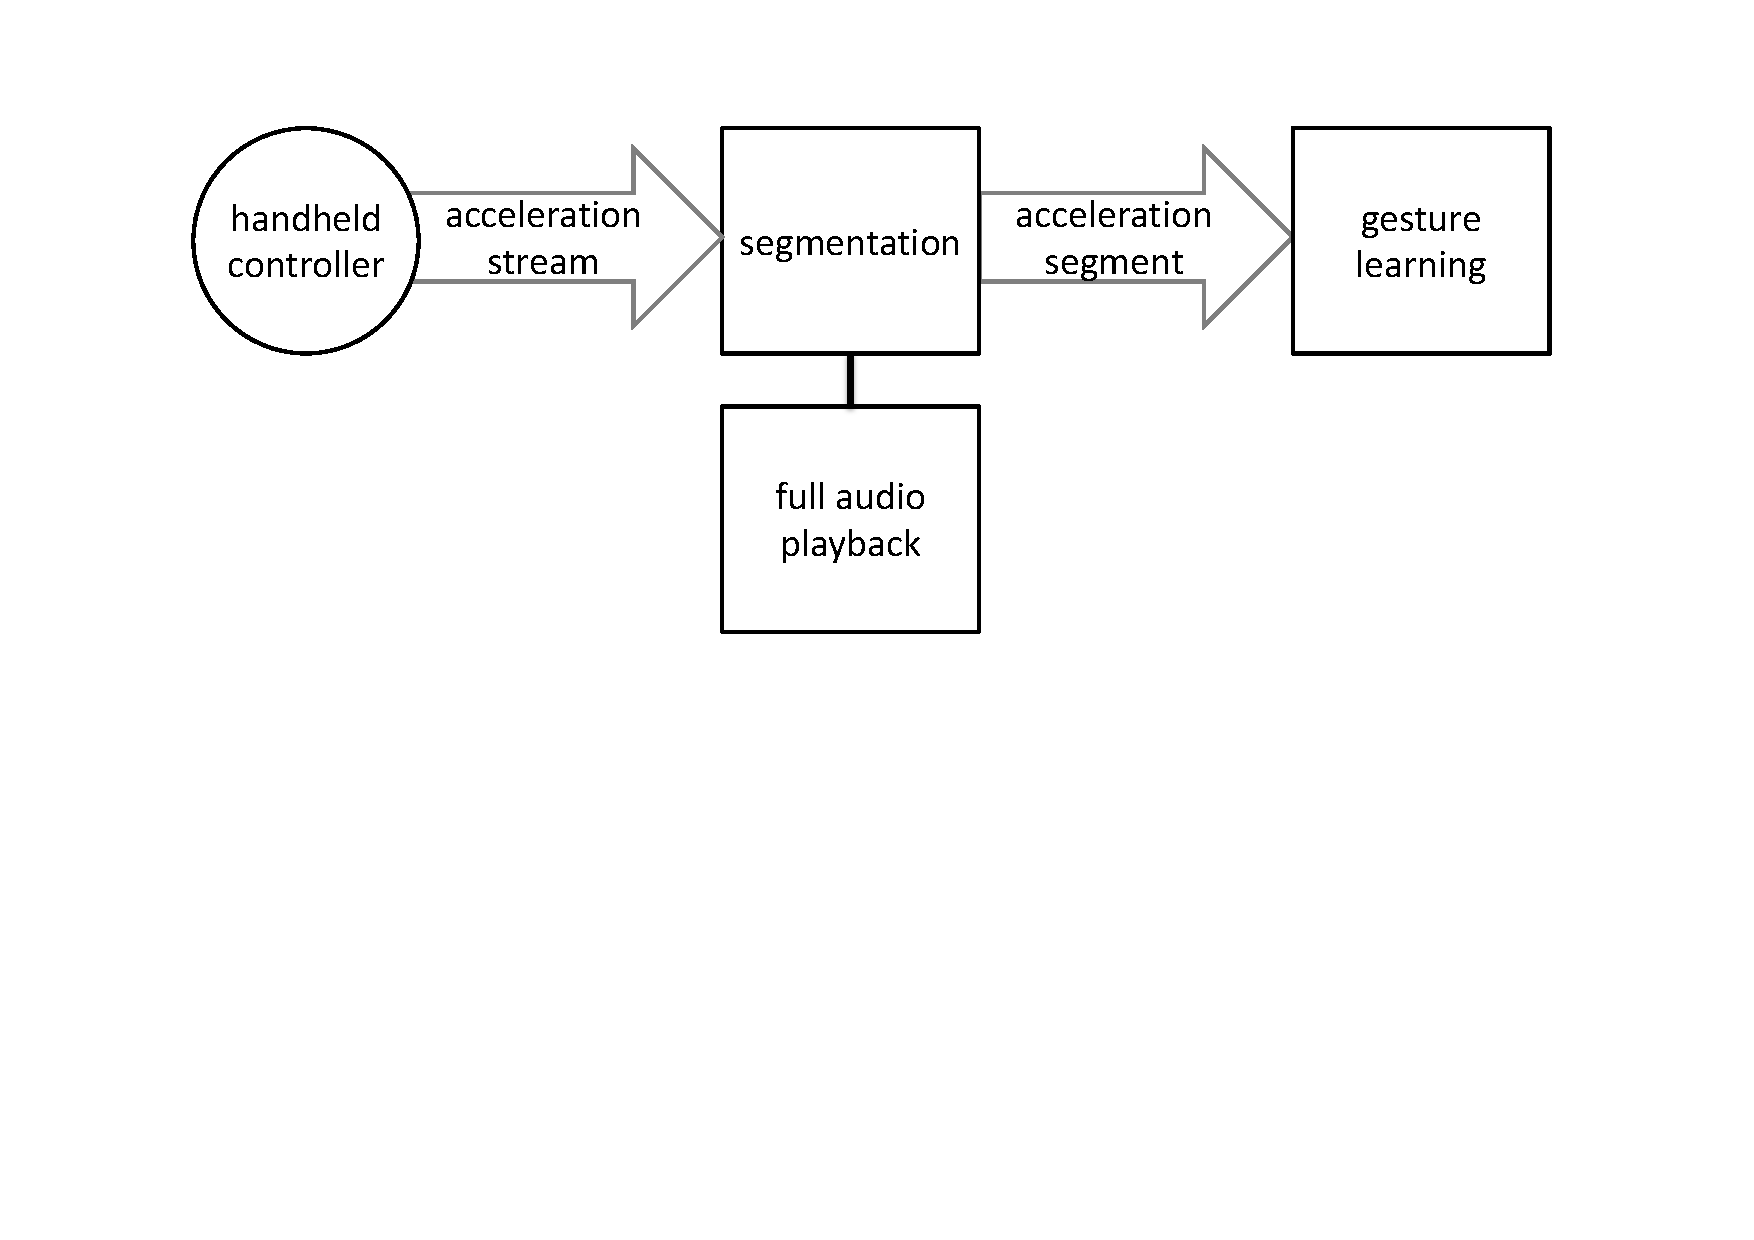
\includegraphics[trim={3.2cm 10.2cm 3.2cm 2.1cm}, clip=true, width=1\columnwidth]{cut}
	\caption{Cut stage}
	\label{fig_3}
\end{figure}

\begin{figure}[t!]
%\vspace{0.3cm}
%\vspace{0.6cm}
	\centering
		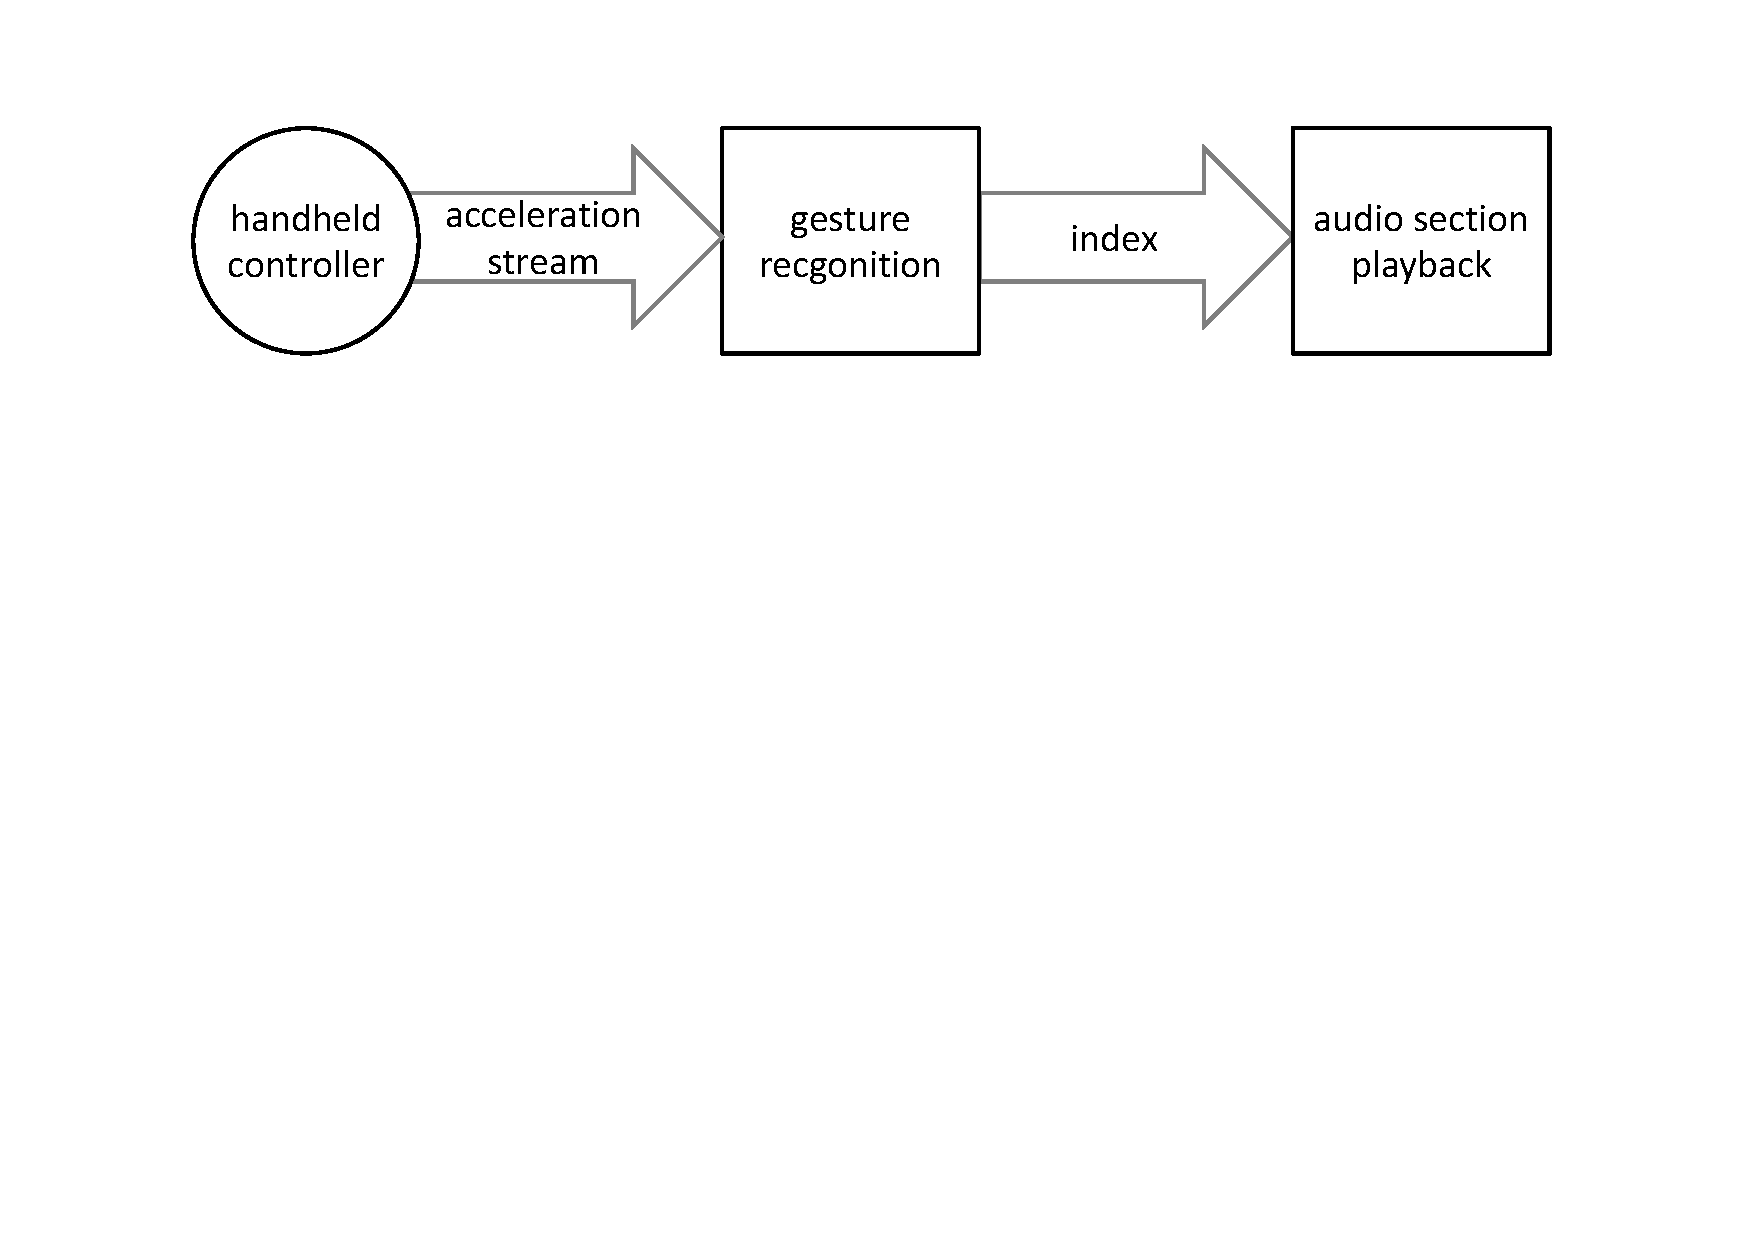
\includegraphics[trim={3.2cm 14.9cm 3.2cm 2.1cm}, clip=true, width=1\columnwidth]{perform}
	\caption{Perform stage}
	\label{fig_4}
%\vspace{0.4cm}
\end{figure}

\begin{figure*}[t!]
%\vspace{0.2cm}
	\centering
		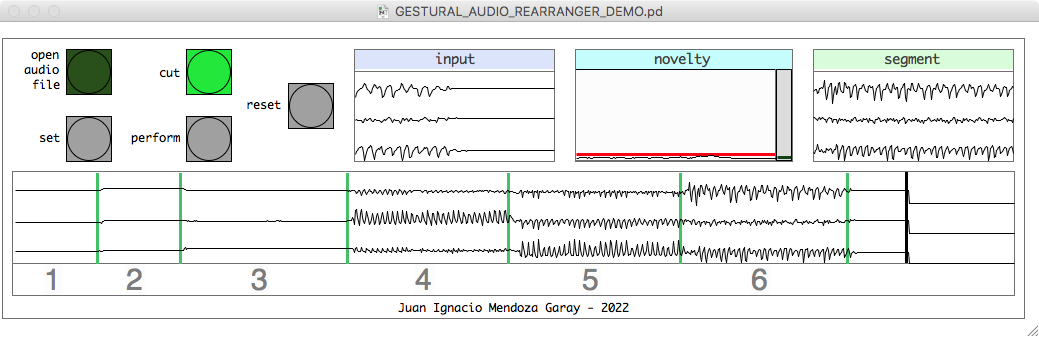
\includegraphics[trim={0.3cm 1.4cm 0.7cm 1.5cm}, clip=true, width=1\textwidth]{GUI_Cut_task}
\caption{Graphical user interface}
%\vspace{0.5cm}
	\label{fig_5}
\end{figure*}

\begin{figure}[t!]
%\vspace{0.2cm}
	\centering
		\includegraphics[width=0.8\columnwidth]{gestures_task_explained}
	\caption{Segmentation task}
	\label{fig_6}
% \vspace{0.2cm}
\end{figure}

%\vspace{0.2cm}

\subsection{Testing}\label{Testing}

During the implementation of the system, the author of this article conducted iterative testing using an upbeat electronic dance music piece, as it has been observed that this kind of music stimulates bodily motion  \cite{Burger_Toiviainen_2020}. Static gestures achieved by only changing the ball's orientation, and gestures involving repetitive motion, were well segmented and recognised.  Figure~\ref{fig_6} shows a sequence of gestures that worked well with the following setting of meta-parameters which was kept throughout the testing: $n = 80$, $n_{min} = 28$, and $n_{filt} = 24$, at a sampling rate of 20 frames per second yielding $lag = 55$ frames (0.4 seconds, not including logical processing latency), and $\theta = 0.03$. Parameters of the DTW process were also adjusted, but are not discussed as that algorithm is well documented \cite{Gillian_etal_2011, Wekinator_website}. Since the ball is fully symmetrical, letters (A to F) were put on the orthogonal points to aid visually in manipulation, and a small arrow was put next to each letter pointing to the next one (Figure~\ref{fig_2}, Right).  

Additionally, extraction of features (e.g., amplitude, zero-crossings) from the triaxial accelerometry signal and its magnitude, was implemented. They did not improve segmentation but, because of being windowed processes, they did increase lag (i.e., frames needed for computation) and computation cost (i.e., logical processing). Therefore, development and testing continued using only raw acceleration, to demonstrate what is possible without using extracted features. 

When a functional version was completed, researchers and students of Musicology, Music Therapy and Music Education at the 
% \anonymize{fooooooooooooooooooooooo}
University of Jyväskylä
were invited to evaluate the functionality of the system. With this group the following protocol was developed:

\textbf{1.}	The researcher demonstrates the task comprising Cut and Perform stages, using the upbeat electronic dance music piece and the tested gestures sequence. The enclosed rectangle shown in Figure~\ref{fig_6} is is displayed on a paper.

\textbf{2.}	The participant is invited to do the task. If in the Cut stage not all gestures were segmented successfully, the participant is invited to repeat the Cut, as many times as they want. Then, they are invited to try the Perform stage.

\textbf{3.}	The participant is invited to freely improvise and/or to use another piece of music.

\textbf{4.}	The participant is invited and encouraged to express their opinion on the experience. The researcher shall take observational notes such as number of gestures correctly segmented in a trial, comments and ideas expressed by and discussed with the participant, and if a new gesture is discovered.

The protocol described above was incorporated to a 7-hour presentation in an outreach event at the 
% \anonymize{fooooooooooooooooooooooo}
University of Jyväskylä. The following data was collected of 23 participants: age, gender, number of gestures successfully segmented consecutively from the first, and observations. Further  notes were taken of more more visitors. All participants used the upbeat electronic dance music, except one  discarded for homogeneity. 17 participants (10 female, 7 male) performed the task as intended. Only six tried a second time, improving segmentation (see Figure~\ref{fig_7}). The medians of correctly segmented gestures was 4 for first time, 6 for second time and 5 for maxima. No correlation between number of correct segments and age or gender was observed. Most participants under 10 years old could not correctly perform all gestures, albeit they could successfully use the system by only changing the orientation of the ball.

\subsection{Overall Assessment}

Any set of orientations being different enough will work, but the 6 orthogonal orientations work flawlessly. Also, any combination and variation of repeated movements along the 3 orthogonal axes of the ball will work well. Sudden and energetic movements work best, as they are better measured by the accelerometer. Smooth movements are less likely to be detected by the system. Participants discovered a variety of gestures beyond those in the task. One of them is the “baby rocking”, consisting in holding the ball with two hands and moving it describing an upwards concave curve. Other semi-circular and circular motions, and ``8" figures were successfully detected, inasmuch as the speed, and therefore radial acceleration, was powerful enough to produce a novelty score above the set threshold ($\theta $).

If the transition from one gesture to the next is slow enough to have a duration equal or greater than meta-parameter $n_{min}$ (minimum duration for gestures to be detected), the transition will be identified as a segment. In the Perform stage the system often will get stuck looping these very short segments, due to the characteristics of the DTW algorithm (i.e., computation time is proportional to the length of the segment). However, interestingly, two participants mentioned that they liked the result. One of them referred to it as “a DJ effect”. Another participant explored the possibility of not having to look at the ball when manipulating it. A discussion ensued leading to conclude that, since the ball is fully symmetric, it is not possible to be aware of its orientation without looking at it.

The task proved to be challenging to different extents. Some participants wanted to try again to improve the number of correctly segmented gestures. All participants showed engagement and enjoyment. However, it is to expect that researchers and students have interest as the experience is related to their profession and studies. Likewise, visitors at the outreach event most probably attended because of curiosity.

\begin{figure}[t!]
%\vspace{0.2cm}
	\centering
		\includegraphics[trim={0.2cm 0.2cm 0.8cm 0.5cm}, clip=true, width=1\columnwidth]{RN_experiment}
	\caption{Data collected at the outreach event. Second trials are shown in darker shade.}
	\label{fig_7}
\end{figure}

\begin{figure}[t!]
	\centering
		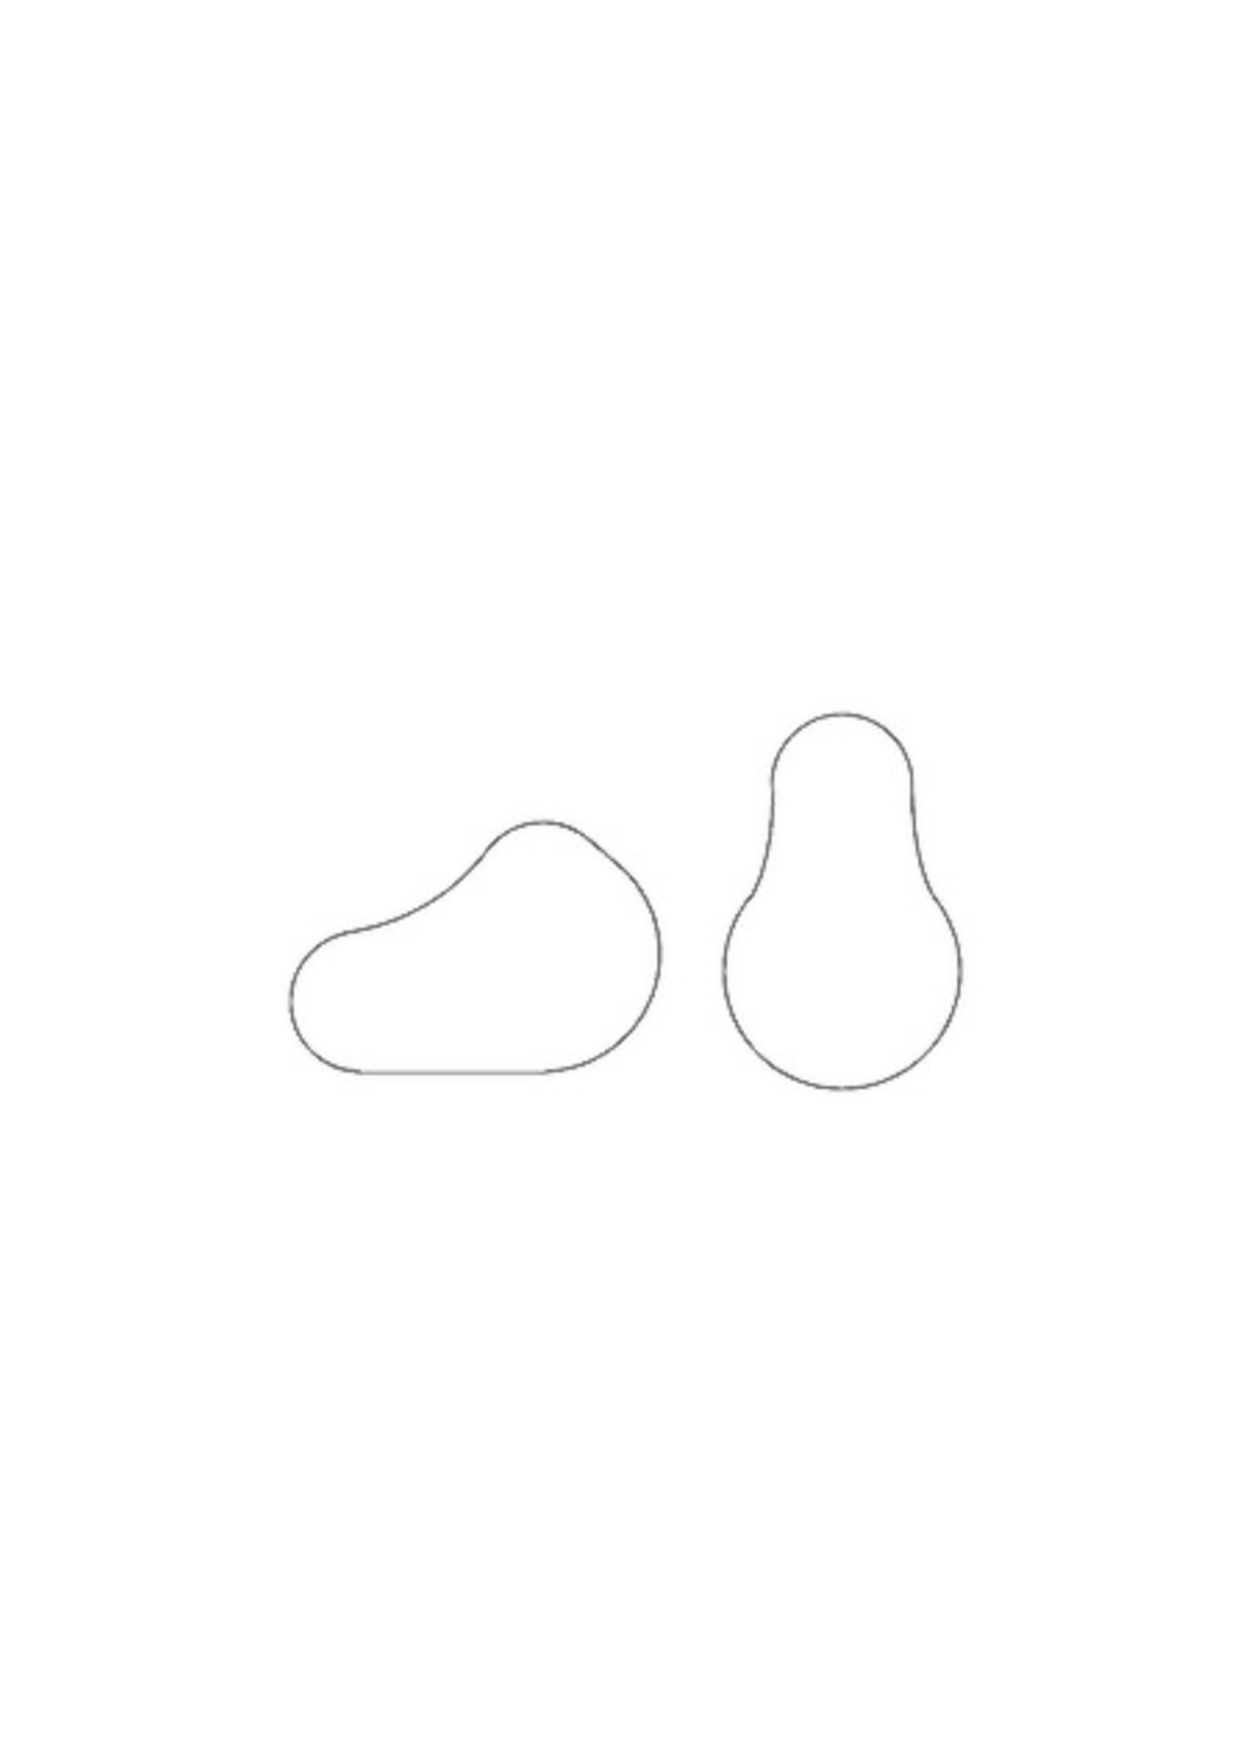
\includegraphics[trim={4cm 11.2cm 4cm 12cm}, clip=true, width=0.5\columnwidth]{boot_shape}
	\caption{"Boot" form with rotational asymmetry. Left -- lateral view. Right -- zenithal view.}
	\label{fig_8}
\end{figure}

\section{Discussion and Future Work}

The system described in this article demonstrates the feasibility of unsupervised learning of patterns in a continuous input signal, for gestural control, within a musical application. The process ineluctably produces a lagged response and therefore it is not suitable for execution of fast notes or rhythmic patterns. Nonetheless, the proposed musical application conforms to this constraint, supporting the concept of delayed control of musical sound. Participants of the assessment tended to regard the task as a challenge, which in combination with the discovery of new meaningful gestures, and the sense-making of the constraints, turned the experience into a ludic one. The system appears promising, offering opportunities for further research:

\textbf{I.} The reported assessment used recorded music, but any audio file may be used, and the meta-parameters may be tweaked for further exploration that may lead to unexpected yet interesting results.

\textbf{II.} Make the hand-held form to have rotational asymmetry, such that there is no need of looking at it for manipulation (Figure \ref{fig_8}).

\textbf{III.}  Using the raw accelerometry signal has established a baseline. Future research could evaluate the impact of features extracted from the raw signal. The computation of such features will impact the overall latency (lag plus logical processing), and the detection of novelty (and therefore the threshold parameter $\theta $) because of the information that the features carry. 

\textbf{IV.}  Incorporation of more sensors or sensing technologies other than accelerometry. Besides, several sensors may be used by more than one person simultaneously, as a group activity (e.g., \cite{Staudt_etal_2022, Tahiroglu_etal_2013}). 

\textbf{V.} Implementation of online multigranular segmentation, meaning the detection of gestural boundaries at different timescales.

\textbf{VI.} Current limitations to achieve \textbf{III}, \textbf{IV}, and \textbf{V}, are algorithmic complexity, processing power and software efficiency. Solutions may include low-level programming (possibly embedded software) and faster hardware (possibly parallel computing of several features and timescales).

\textbf{VII.} The setting of meta-parameters generalised well, which is unexpected as perceptual evaluations have suggested the adjustment of meta-parameters for each user 
% \anonymize{foooooooooooooooooo}
Mendoza \cite{Mendoza_2022}. 
A different setting might be needed when using other configurations of hardware, software, music, user, etc. Future research may assess the effects of meta-parameters on segmentation and user experience.

\textbf{VIII.} The methods described in this article have potential beyond the described application, in which the online segmentation procedure only contributes to display on the screen an indication when a gesture has been successfully segmented in the Cut stage. This allows the user, for example, to stop the Cut and restart if a gesture change was not detected. While this might be an advantage to the user, the online segmentation capability and its further possibilities for near-real-time interaction could be exploited more. For example, a musical system (e.g., a DMI, a sonic installation, a sonification) may learn gestures as they occur. This may be incorporated to interactive systems where both the user and the system discover and learn gestures at the same time, leading to a seamless process of human-machine musical interaction.

%\end{document}  % This is where a 'short' article might terminate

\section{Ethical Standards}
All participants gave verbal informed consent for the use of their anonymous collected data, following the research ethics guidelines by the 
% \anonymize{fooooooooooooooooooooooo}
University of Jyväskylä.

%
% The following two commands are all you need in the
% initial runs of your .tex file to
% produce the bibliography for the citations in your paper.
\bibliographystyle{abbrv}

	\bibliography{delayed_control_unsupervised_segmentation_SHORT_NIME_2023} 

% You must have a proper ".bib" file
%  and remember to run:
% latex bibtex latex latex
% to resolve all references
%
% ACM needs 'a single self-contained file'!
%
%APPENDICES are optional
\appendix
Software and documentation: 
\href{https://gitlab.jyu.fi/juigmend/temporal_segmentation_gestural_control}{https://gitlab.jyu.fi/juigmend\\/temporal\_segmentation\_gestural\_control}
% \anonymize{fooooooooooooooooooooooo}

%%Appendix A
%\section{Headings in Appendices}
%The rules about hierarchical headings discussed above for
%the body of the article are different in the appendices.
%In the \textbf{appendix} environment, the command
%\textbf{section} is used to
%indicate the start of each Appendix, with alphabetic order
%designation (i.e. the first is A, the second B, etc.) and
%a title (if you include one).  So, if you need
%hierarchical structure
%\textit{within} an Appendix, start with \textbf{subsection} as the
%highest level. Here is an outline of the body of this
%document in Appendix-appropriate form:
%\subsection{Introduction}
%\subsection{The Body of the Paper}
%\subsubsection{Type Changes and  Special Characters}
%\subsubsection{Math Equations}
%\paragraph{Inline (In-text) Equations}
%\paragraph{Display Equations}
%\subsubsection{Citations}
%\subsubsection{Tables}
%\subsubsection{Figures}
%\subsubsection{Theorem-like Constructs}
%\subsubsection*{A Caveat for the \TeX\ Expert}
%\subsection{Conclusions}
%\subsection{Acknowledgments}
%\subsection{Additional Authors}
%This section is inserted by \LaTeX; you do not insert it.
%You just add the names and information in the
%\texttt{{\char'134}additionalauthors} command at the start
%of the document.
%\subsection{References}
%Generated by bibtex from your ~.bib file.  Run latex,
%then bibtex, then latex twice (to resolve references)
%to create the ~.bbl file.  Insert that ~.bbl file into
%the .tex source file and comment out
%the command \texttt{{\char'134}thebibliography}.
%
%
%% This next section command marks the start of
%% Appendix B, and does not continue the present hierarchy
%\section{More Help for the Hardy}
%The sig-alternate.cls file itself is chock-full of succinct
%and helpful comments.  If you consider yourself a moderately
%experienced to expert user of \LaTeX, you may find reading
%it useful but please remember not to change it.

%%% Place this command where you want to balance the columns on the last page. 
%\balancecolumns 

% That's all folks!
\end{document}
